\chapter{InterSense InertiaCube3}
\label{AppendixD}
\lhead{Appendix D. \emph{InterSense InertiaCube3}}

\begin{figure}[htbp]
  \centering
    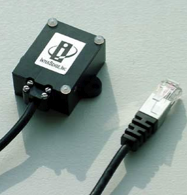
\includegraphics{./Primitives/inertiacube3.png}
    \rule{35em}{0.5pt}
  \caption[InterSense InertiaCube3]{InterSense InertiaCube3}
\end{figure}

\begin{itemize}
	\item Degrees of Freedom: 3 (Yaw, Pitch and Roll) 
	\item Angular Range Full: 360° - All Axes 
	\item Maximum Angular Rate*: 1200° per second 
	\item Minimum Angular Rate*: 0° per second 
	\item RMS Accuracy*: 1° in yaw, 0.25° in pitch and roll at 25°C 
	\item RMS Angular Resolution*: 0.03° 
	\item Serial Interface Update Rate: 180 Hz 
	\item Minimum Latency: 2 ms for RS-232 (PC host OS dependent) 
	\item Prediction: up to 50 milliseconds 
	\item Serial Rate: 115.2 kbaud 
	\item Interface: RS-232 Serial (shown above) 
	\item Size: (without mounting plate) 1.031 in x 1.544 in x 0.581 in (26.2 mm x 39.2 mm x 14.8 mm) 
	\item Weight: 0.6 ounces (17.0 grams) 
	\item Cable Length: 15 ft. (4.572 m) - Max. 75 ft (22.86 m) 
	\item Power: 6 VDC, 40 ma 
	\item Operating Temperature Range: 0° to 70° C 
	\item O/S Compatibility: .dll for Windows Vista/XP/2000, .so for Linux 
	\item Software Support: SDK with full InterSense API, Ethernet via Windows Control Software, Heading Calibration Software
\end{itemize}
